\documentclass[conference]{IEEEtran}
\IEEEoverridecommandlockouts
\usepackage{cite}
\usepackage{amsmath,amssymb,amsfonts}
\usepackage{graphicx}
\usepackage{textcomp}
\usepackage{xcolor}
\usepackage{url}
\usepackage{booktabs}
\usepackage{array}
\usepackage{hyperref}
\usepackage[ruled,linesnumbered]{algorithm2e}
\graphicspath{{figures/}}

\begin{document}

\title{Improving the Availability of Binance Market Data under Reconnection Storms through the RelayBook Architecture with State-Based Resume}

\author{\IEEEauthorblockN{Nicolas Diego Castaneda Quichis}
\IEEEauthorblockA{nicolas.castaneda@utec.edu.pe \\ 100\%}
\and
\IEEEauthorblockN{Pedro Enrique Mori Ortiz}
\IEEEauthorblockA{pedro.mori@utec.edu.pe \\ 100\%}
}

\maketitle

\begin{abstract}
Binance distributes order book market data over WebSocket to millions of clients. Its documented recovery contract requires every client that loses its connection to request a full snapshot through a rate-limited REST endpoint. During a volatility spike with correlated disconnections, this recovery work competes with the live stream for the same capacity, a feedback loop with the structure of a metastable failure. This paper studies the Binance contract and proposes RelayBook, an architecture of regional relays in which a reconnecting client receives only the price levels that changed since its last sequence number. The hypothesis is that the public Binance contract can remain degraded after a spike ends, while RelayBook, whose recovery cost is bounded by the number of changed price levels, returns to a healthy state on its own. The architecture separates distribution from recovery, resumes clients from the state of the book instead of the log of missed messages, and conflates updates for slow clients. A prototype of the relay recovered every client with a correct book on 70 minutes of real Binance traffic, and reduced the recovery payload by 63\% against a snapshot after a 1\,s disconnection. In a simulated reconnection storm with 2\,000 clients, RelayBook recovered immediately and kept the origin load at 0.3\,MB/s against 120\,MB/s under the Binance contract, while the Binance contract failed to recover only when generating a snapshot was expensive for the origin. The hypothesis was refuted for the share of full resynchronizations, since during the spike every RelayBook recovery required a full snapshot from its relay.
\end{abstract}

\begin{IEEEkeywords}
market data dissemination, order book resynchronization, metastable failures, reconnection storm, overload control, software architecture
\end{IEEEkeywords}

\section{Introduction}

An exchange publishes market data so that each client can keep a local copy of the order book. Binance sends an initial snapshot followed by incremental updates with sequence numbers. When a client loses its connection, the stream does not replay the missed updates, so the client must request the full book again through a REST endpoint protected by rate limits and bans \cite{binance-localbook,binance-streams}.

If many clients disconnect at the same time, the recovery requests compete with the live stream, which may cause further disconnections. When this loop keeps the system degraded after the original spike ends, the failure is known as metastable \cite{isaacs2025}. The objective of this work is to analyze that risk in the public Binance contract and to propose RelayBook, an architecture intended to keep recovery work away from the origin, whose effect is stated as a hypothesis to be tested experimentally.

\section{Background}

\subsection{Order Book and Market Data}

An order book lists the pending buy and sell orders of an instrument such as BTC/USDT, and each price level groups all orders at the same price. Market data is published at three levels of detail. L1 contains only the best bid and ask, L2 contains every price level with its aggregated quantity, and L3 contains every individual order. Binance publishes L2 through its \texttt{depth} stream, where each update carries the absolute quantity of each modified price level and a quantity of zero removes the level. A client that detects a gap in the sequence numbers must discard its book and request a new snapshot \cite{binance-localbook}.

\subsection{Metastable Failures}

A metastable failure is a degraded state that persists after its trigger is removed, because a sustaining effect such as a retry storm prevents the system from draining its backlog \cite{isaacs2025}. Unlike a regular overload, the system does not recover when the load returns to normal, and recovery usually requires manual intervention such as shedding load or restarting components.

\section{State of the Art}
\label{sec:sota}

The migration of financial exchanges to the public cloud has motivated architectures that deliver market data without network multicast. Jasper builds an overlay multicast tree of proxies that delivers market data to about 1\,000 participants with low latency and small differences in reception time, and reports around 50\% lower latency than the multicast service of AWS \cite{onyx2024}. DBO provides fairness among participants of cloud-hosted exchanges through delivery-based ordering \cite{dbo2023}. These works place intermediate nodes between the exchange and its clients, as RelayBook does, but they optimize fair and simultaneous delivery to a bounded set of market participants and do not address how a disconnected client recovers its book.

Research on metastable failures has moved from describing them to predicting them. Isaacs et al. combine queueing models, discrete-event simulation and emulation to predict when a service becomes vulnerable to this kind of failure \cite{isaacs2025}. Farahbakhsh et al. propose a simple model that explains and predicts metastable states in data-center systems \cite{farahbakhsh2025}, and later trace these failures to cycles of interaction between components that are stable in isolation, which scheduling decisions turn into failures \cite{characterizing2026}. These works provide the analysis framework of this paper, although none of them studies the dissemination of state to clients.

Overload control offers tactics against the same loops. RetryGuard adjusts the retry policy of each service to reduce retry storms in microservices \cite{retryguard2025}, and Rajomon attaches tokens to requests and prices to APIs to drop requests in a decentralized way \cite{rajomon2025}. Both protect the service by limiting or discarding work. In market data, a delayed or discarded resynchronization leaves the client with an invalid book, so these tactics are not expected to restore the service from the point of view of the client.

In practice, Kraken sends the snapshot over the same WebSocket channel when a client subscribes and requires the client to discard its local book after a reconnection \cite{kraken-reconnect}, Ably resumes a connection from the last received serial within a two-minute window \cite{ably-states}, and CME publishes a looping snapshot on a separate recovery feed that relies on multicast over private networks \cite{cme-recovery}. In the WebSocket-based contracts, the total recovery work grows with the number of disconnected clients, and in the serial-based case it also grows with the message rate. None of the reviewed works bounds the cost of recovering a client by the number of price levels that changed during its disconnection, and none analyzes market data recovery as a possible metastable failure.

\section{Study of the Binance Case}
\label{sec:study}

The documented contract allows a feedback loop. A volatility spike multiplies the message rate, the connections of slow clients close, each of those clients requests a full REST snapshot, and the server may delay the stream while serving those snapshots, which can close further connections. Two documented rules may amplify the loop, since further requests after an HTTP 429 response lead to an HTTP 418 ban and repeatedly disconnected IPs may be banned \cite{binance-general,binance-streams}.

Users of the official developer forum report connections closing with code 1006 during heavy trading and many depth streams closing at the same time \cite{forum-1006,forum-depth}. Tardis.dev, a provider of historical market data, documents that it rebuilds the book from the REST snapshot after detecting a missed message in the Binance stream \cite{tardis-binance}.

No public post-mortem attributes a Binance incident to this loop, and the internal mitigations of Binance are unknown. This paper therefore claims only that the public contract meets the structural conditions of a metastable failure, and treats its actual behavior as a question to be tested through simulation.

\section{Requirements}

\subsection{Functional Requirements}

\begin{itemize}
\item FR1. The system delivers L2 updates in order, with sequence numbers.
\item FR2. A reconnecting client can resume from its last sequence number.
\item FR3. A client without a valid sequence number can obtain a full snapshot.
\item FR4. Slow clients are served without being disconnected.
\end{itemize}

\subsection{Non-Functional Requirements}

\begin{itemize}
\item NFR1. During a spike, less than 1\% of the reconnections end in a full snapshot.
\item NFR2. After a spike, 99\% of the clients hold a valid book within 30\,s, without manual intervention.
\item NFR3. The p99 staleness of the client book stays below 1\,s during a spike.
\end{itemize}

\section{User Model}

Three users drive the requirements, described in Table~\ref{tab:users}.

\begin{table}[t]
\caption{User model}
\label{tab:users}
\centering
\footnotesize
\begin{tabular}{p{1.8cm}p{2.7cm}p{2.7cm}}
\toprule
User & Context & Need \\
\midrule
Retail trader on mobile & Unstable network, frequent reconnections & Correct prices right after reconnecting \\
Trading bot or market maker & Many instruments, automated reconnection & Fast resynchronization without bans \\
Exchange operator & Responsible for availability & Automatic recovery after spikes \\
\bottomrule
\end{tabular}
\end{table}

\section{Proposed Architecture}

RelayBook follows a hierarchical, push-based publish-subscribe style. Fig.~\ref{fig:arch} contrasts it with the public Binance contract. In the Binance contract every reconnection ends in a request to the origin, while in RelayBook the origin publishes a single sequenced feed to a tier of regional relays, and reconnections are resolved at the relays.

\begin{figure*}[t]
\centering
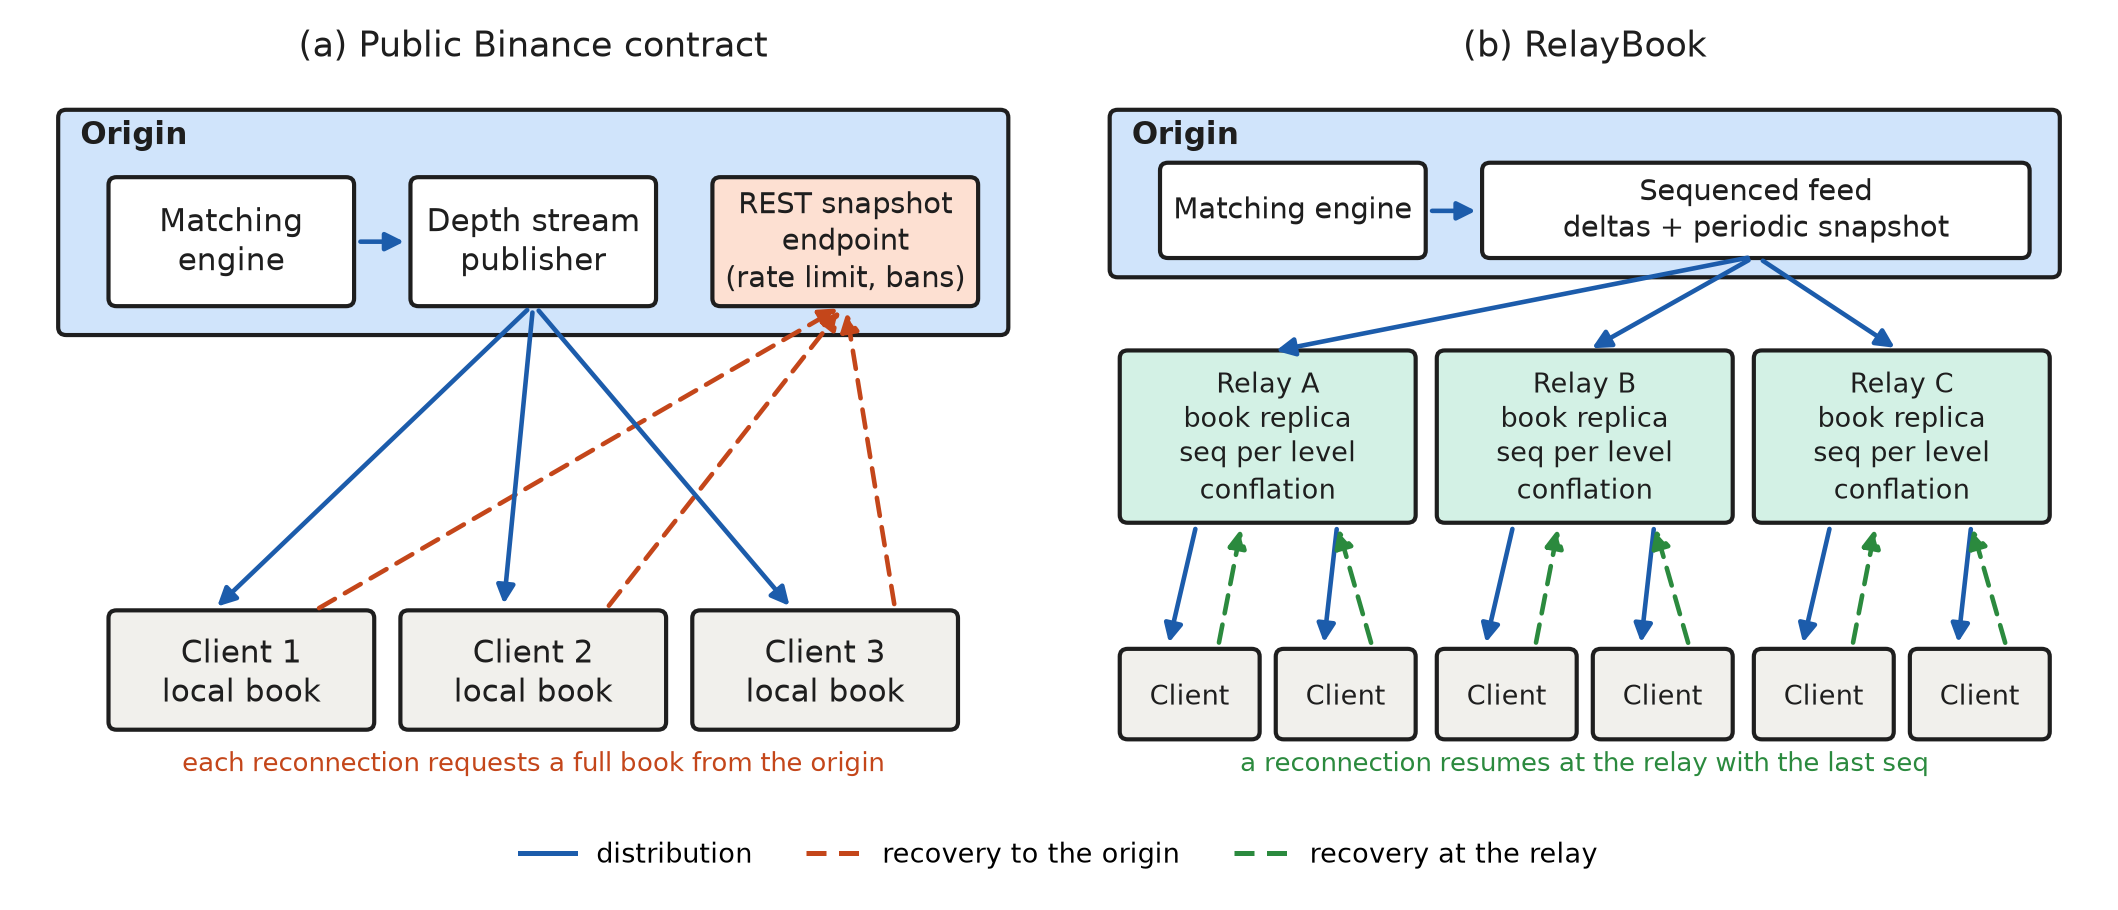
\includegraphics[width=\textwidth]{architecture.png}
\caption{Recovery paths in the public Binance contract (a) and in RelayBook (b).}
\label{fig:arch}
\end{figure*}

\subsection{Components}

The origin contains the matching engine and a sequencer that publishes, for each instrument, a feed of L2 deltas with consecutive sequence numbers. The same feed carries a full snapshot of the book every $T$ seconds. The origin only accepts connections from relays, so its fan-out depends on the number of relays $R$ and not on the number of clients $N$.

Each relay subscribes to the feed, applies every delta to a replica of the book and stores, for every price level, the sequence number of its last change. Removed levels are kept as tombstones with quantity zero until a retention horizon $S_{min}$, so that a resuming client also learns which levels disappeared. A relay that detects a gap in the feed discards its replica and waits for the next periodic snapshot instead of requesting one from the origin.

Each client keeps its local book and the sequence number of the last delta it applied. Since sequence numbers are assigned by the origin, a client can resume at any relay whose retention horizon covers its last sequence number, which allows a client to move to another relay if its own relay fails.

\subsection{State-Based Resume}

Algorithm~\ref{alg:resume} describes how a relay answers a reconnecting client. If the relay is resynchronizing after a gap in the feed, it redirects the client to another healthy relay of the region, or holds the client until the next periodic snapshot when no healthy relay is available. If the last sequence number of the client is newer than the replica, which happens when the client comes from a faster relay, the relay waits until its replica reaches that sequence number, so that a client never moves backward in time. If the last sequence number of the client is older than the retention horizon, the relay sends a full snapshot from its own replica. Otherwise it sends only the levels whose last change is newer than that sequence number, with their current quantity. Because each quantity is absolute, applying the current value of a level is equivalent to applying all of its intermediate changes, and the size of the response is bounded by the number of distinct levels changed during the disconnection, which never exceeds the size of the book plus its tombstones. If the relay keeps its levels in an index ordered by their last sequence number, the set $D$ is obtained in time proportional to its size. The set $D$ is restricted to the levels visible to the client, that is, every level better than the deepest level of the snapshot depth on each side. The restriction keeps the tombstones left on the other side of the best price when the price moves, which must reach the client to remove levels that no longer exist. When the size of $D$ reaches the size of a snapshot, the relay sends the snapshot instead, so a resume never costs more than a full resynchronization.

Consider a client that misses five updates while disconnected, in which level 67\,000 is set to 1.0, 1.5, 0.7 and 1.2~BTC and level 66\,999 is set to 0.8~BTC. Under the Binance contract the client downloads the full book from the origin, which may contain hundreds of levels. Under a serial-based resume in the style of Ably \cite{ably-states} it receives the five missed messages. Under state-based resume it receives only two levels, 67\,000 at 1.2~BTC and 66\,999 at 0.8~BTC, because the last value of a level replaces the previous ones. Table~\ref{tab:recovery} summarizes the three contracts. During a spike the number of messages is expected to grow much faster than the number of distinct levels they modify, since updates concentrate near the best price.

\begin{table}[t]
\caption{Cost of recovering a reconnecting client}
\label{tab:recovery}
\centering
\footnotesize
\begin{tabular}{p{1.5cm}p{3.1cm}p{2.6cm}}
\toprule
Contract & What the client receives & Cost grows with \\
\midrule
Binance & Full book, through REST from the origin & Disconnected clients, one full book each \\
Ably-style resume & Every missed message, within a two-minute window & Message rate and disconnection time \\
RelayBook & Current value of each changed level, from the relay & Distinct changed levels, bounded by book depth \\
\bottomrule
\end{tabular}
\end{table}

\begin{algorithm}[t]
\caption{State-based resume at a relay}
\label{alg:resume}
\KwData{Relay book $B$ with entries $(p, q_p, s_p)$, current sequence $S$, retention horizon $S_{min}$, last client sequence $s_c$}
\KwResult{Resume message for the client}
\If{the replica has a gap in the feed}{
  \lIf{another relay of the region is healthy}{\Return redirect to that relay}
  wait for the next periodic snapshot\;
}
\If{$s_c > S$}{
  wait until $S \geq s_c$\;
}
\eIf{$s_c < S_{min}$}{
  \Return full snapshot of $B$ tagged with $S$\;
}{
  $D \leftarrow \{(p, q_p) \mid (p, q_p, s_p) \in B,\ s_p > s_c,\ p \text{ visible}\}$\;
  \lIf{$|D|$ reaches the size of a snapshot}{\Return full snapshot of $B$ tagged with $S$}
  \Return delta $D$ tagged with the range $(s_c + 1, S)$\;
}
\end{algorithm}

\subsection{Slow-Client Conflation}

Each client connection has a bounded queue. While the queue has space, the relay forwards deltas unchanged. When the queue is full, the relay stops enqueuing deltas and merges new changes into a pending map from price level to latest quantity, together with the first and last sequence numbers it covers. When the connection becomes writable again, the relay sends the pending map as a single delta with that sequence range. The client applies it as a normal delta, so a slow client receives fewer intermediate updates instead of losing its connection.

\subsection{Replication and Consistency}
\label{sec:replication}

RelayBook applies leader-follower replication. The origin acts as the leader, the relays act as followers and the sequenced feed acts as the replication log. Each relay holds exactly the book of the origin at some sequence number, possibly a few milliseconds behind, which corresponds to eventual consistency with consistent prefixes. A relay may serve stale data, whose delay is measured as staleness, but it must never serve a book that did not exist at the origin. The delay of a relay is its replication lag, defined as the difference between the last sequence number published by the origin and the last one applied by the relay.

Four mechanisms support this property. Only the origin assigns sequence numbers, so every relay applies the same log in the same order. A relay that detects a gap stops answering resumes until the next periodic snapshot, and redirects its reconnecting clients to another healthy relay of the region or holds them when no such relay is available. Clients verify the continuity of the sequence numbers they receive, as the Binance contract already requires \cite{binance-localbook}. Finally, the feed periodically carries a checksum of the top levels of the book, similar to the CRC32 over the top ten levels used by Kraken \cite{kraken-book}, which relays and clients compare with their own book to detect divergence.

The replication lag is measured and bounded instead of eliminated. Each relay reports its lag, and when the lag exceeds an initial threshold of 500\,ms, half of the staleness target of NFR3, the relay marks itself unhealthy and stops accepting new resumes, so that reconnecting clients move to another relay of the region. The period $T$ of the snapshot bounds the time a relay stays without a valid replica after a gap, and is initially set to 1\,s, since an L2 snapshot of a single instrument is in the order of tens of kilobytes.

Each relay replicates the most traded instruments at all times, since they concentrate most of the traffic during a spike. Less traded instruments are subscribed when the first client of the relay requests them and released after a period without clients, and that first client waits up to $T$ for the snapshot. When a relay cannot sustain the deltas of its instruments, the instruments of the region are partitioned among several relay nodes. The prototype replicates a single instrument, BTC/USDT.

\subsection{Architectural Decisions and Trade-Offs}

Separating the distribution path from the recovery path is intended to make the work of the origin independent of the number of disconnected clients. The cost is a new tier of relays that must be deployed and operated, and that becomes a failure point for its region, mitigated by the ability of clients to resume at another relay. Leader-follower replication introduces a replication lag between the origin and each relay, which adds to the staleness observed by clients and is bounded by the health threshold of each relay. Redirecting or holding clients during a gap in the feed trades a longer resume for the correctness of the book, and on-demand subscription trades the waiting time of the first client of a less traded instrument for the memory of the relay. Storing the last sequence number per level and the tombstones increases the memory of each relay, and conflation trades the completeness of intermediate updates for the continuity of the connection.

\subsection{Hypothesis}

The hypothesis has two parts. First, the public Binance contract, simulated with real traffic replayed at 10x, remains degraded after the spike ends. Second, under the same conditions RelayBook is expected to keep full resynchronizations below 1\% of the reconnections, to return to a healthy state within 30\,s without manual intervention and to keep the p99 staleness below 1\,s, while the Ably-style resume is expected to show higher staleness during the spike, because each recovery carries every missed message. Either part may be refuted by the measurements.

\section{Evaluation Metrics}

Table~\ref{tab:metrics} lists the metrics selected to test the hypothesis. Each metric corresponds to one non-functional requirement and is defined as a fitness function with an initial threshold, so that the experiment can decide automatically whether the requirement holds.

\begin{table}[t]
\caption{Evaluation metrics}
\label{tab:metrics}
\centering
\footnotesize
\begin{tabular}{p{1.6cm}p{3.6cm}p{1.6cm}}
\toprule
Metric & Definition & Target \\
\midrule
Full resync ratio & Reconnections that end in a full snapshot over all reconnections during the spike (NFR1) & $< 1\%$ \\
Time to recover & Time from the end of the spike until 99\% of clients hold a valid book (NFR2) & $\leq 30$\,s, no manual action \\
Staleness p99 & Delay between an update at the origin and its application at the client, during the spike (NFR3) & $< 1$\,s \\
\bottomrule
\end{tabular}
\end{table}

The first part of the hypothesis holds if, for the Binance contract, the time to recover exceeds the observation window, that is, if fewer than 99\% of the clients hold a valid book at the end of the final phase at normal rate. The second part holds if RelayBook meets every target of Table~\ref{tab:metrics} under the same traffic.

The scenario replays a recording of the Binance \texttt{depth} stream in three phases, five minutes at normal rate, five minutes at 10x with correlated disconnections of a share of the clients, and ten minutes at normal rate. Clients follow fast and slow network profiles. The same scenario is applied to RelayBook and to two baselines described in Section~\ref{sec:sota}, the public Binance contract and the Ably-style resume from the last received serial within a two-minute window.

\section{Implementation}

\subsection{Data}

A recorder subscribed to the public \texttt{btcusdt@depth@100ms} stream of Binance USD-M Futures and took a REST snapshot of 1\,000 levels per side, following the documented procedure \cite{binance-localbook}. The recording started on 13 November 2026 at 09:12 (UTC$-$5) and lasted 70 minutes, with 41\,113 messages and no gap in the sequence numbers. The stream carried 9.8 messages per second with a mean size of 5.8\,KB and a p99 of 29\,KB, and each message updated 275 price levels on average. The snapshot contained 2\,000 levels and weighed 41\,KB.

\subsection{Prototype and Simulator}

The relay was implemented in Python following Algorithm~\ref{alg:resume}. It applies the recorded feed to a replica of the book, keeps the sequence number and the tombstone of every level, restricts each resume to the visible levels, replaces the delta by a snapshot when the delta is larger, and computes a CRC32 checksum over the ten best levels of each side. During its validation, a first version restricted the delta to the levels between the best price and the deepest visible level, which left removed levels on the other side of the best price in the client book. The checksum exposed the error, and the visible band was redefined as every level better than the deepest visible level.

The reconnection storm was evaluated with a discrete-time simulator written in Python with NumPy, an approach close to the simulation-based analysis of metastable failures proposed by Isaacs et al. \cite{isaacs2025}. Each tick lasts 100\,ms and publishes the recorded messages that correspond to the current phase. Every server has an egress capacity in bytes per tick that is shared among its flows with max-min fairness, and every client has its own downlink rate. The recovery work of each design follows Table~\ref{tab:recovery}, and the payload of a state-based resume is obtained from the number of distinct visible levels changed in the recording for the same number of missed messages. Table~\ref{tab:params} lists the parameters. The capacity of each server is expressed as a multiple $h$ of the load of the stream at normal rate for the clients it serves, and is swept between 1.5 and 15. Since the cost of generating a REST snapshot at the origin is not public, it is swept at 1, 10 and 50 times the cost of sending its bytes.

\begin{table}[t]
\caption{Simulation parameters}
\label{tab:params}
\centering
\footnotesize
\begin{tabular}{p{4.6cm}p{2.6cm}}
\toprule
Parameter & Value \\
\midrule
Clients and relays & 2\,000 and 3 \\
Phases & 5 min at 1x, 5 min at 10x, 10 min at 1x \\
Clients disconnected at the start of the spike & 30\%, back after 1 to 5\,s \\
Client downlink & 70\% at 2\,MB/s, 30\% at 80\,KB/s \\
Output buffer before closing a connection & 1\,MB \\
Backlog before conflation (RelayBook) & 256\,KB \\
Reconnection when the book is older than & 5\,s \\
Retry of a recovery that does not arrive & 10\,s \\
Resume window (Ably-style) & 2 min \\
\bottomrule
\end{tabular}
\end{table}

\subsection{Technology Choices}

The prototype uses Python 3.13 with NumPy and Matplotlib, and the \texttt{websockets} library for the recorder, because the experiments depend on processing a large recording and on reproducing thousands of clients deterministically within the time available. A production deployment would require a different stack, which this work did not build or measure. Relays are network services that hold many concurrent WebSocket connections, so a runtime with efficient concurrent input and output, such as Go, is a natural candidate, and the feed between the origin and the relays requires an ordered and replayable log per instrument.

\section{Scaled Architecture}

The load of the origin follows directly from the recording. Under the Binance contract the origin sends the stream to every client, about 57\,KB/s per client and instrument at normal rate. Under RelayBook the origin sends the stream and the periodic snapshot to every relay, about 98\,KB/s per relay and instrument with $T = 1$\,s, independent of the number of clients. Table~\ref{tab:scale} estimates both loads for one instrument at normal rate, assuming relays with a 10\,Gb/s network interface and a capacity of three times their normal load, which gives about 7\,000 clients per relay. During a spike both loads grow with the message rate, but the load of the origin under RelayBook still depends only on the number of relays. Beyond one instrument, relays are partitioned by instrument as described in Section~\ref{sec:replication}, and regions are added by deploying relays close to the clients.

\begin{table}[t]
\caption{Estimated origin load for one instrument at normal rate}
\label{tab:scale}
\centering
\footnotesize
\begin{tabular}{p{1.4cm}p{1.9cm}p{1.3cm}p{2.0cm}}
\toprule
Clients & Binance origin & Relays & RelayBook origin \\
\midrule
$10^4$ & 0.55\,GB/s & 2 & 0.2\,MB/s \\
$10^5$ & 5.5\,GB/s & 14 & 1.3\,MB/s \\
$10^6$ & 55\,GB/s & 140 & 13\,MB/s \\
\bottomrule
\end{tabular}
\end{table}

\section{Results}

\subsection{Recovery Payload and Correctness}

Fig.~\ref{fig:payload} shows the payload of a recovery measured on the recording for disconnections between 1 and 60\,s at normal rate. A state-based resume required 15\,KB after 1\,s and 31\,KB after 3\,s, 63\% and 24\% less than the 41\,KB of a snapshot. Between 5 and 10\,s the number of distinct visible levels changed reached the size of the snapshot, so the relay sent the snapshot instead. A log-based resume required 44\,KB after 1\,s and grew to 3.4\,MB after 60\,s. The gap between messages and distinct levels grows with the duration of the disconnection, since a client that misses 10\,s receives about 27\,000 level updates that touch only 2\,770 distinct visible levels, and after 100\,s the difference reaches a factor of 61. Across 46 random reconnections, every client book matched the book of the relay both in its checksum and in its 100 best levels per side.

\begin{figure}[t]
\centering
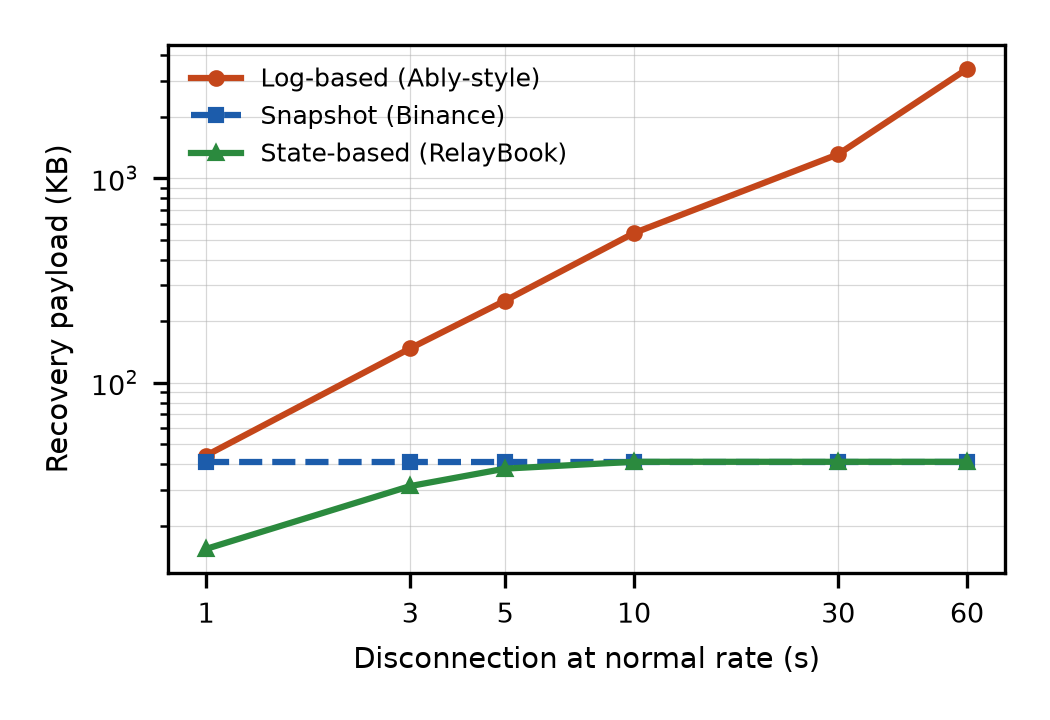
\includegraphics[width=\columnwidth]{e1_payload.png}
\caption{Recovery payload measured on the Binance recording for each recovery contract.}
\label{fig:payload}
\end{figure}

\subsection{Reconnection Storm}

Table~\ref{tab:results} reports the three metrics for a capacity of three times the normal load, and Fig.~\ref{fig:valid} shows the share of clients with a valid book over time. Under the Binance contract with a snapshot cost equal to its bytes, clients disconnected and reconnected repeatedly during the spike, but 99\% of them held a valid book again within 11\,s of its end at every capacity. When the snapshot cost ten times its bytes, the contract did not recover within the ten minutes of observation with a capacity of 1.5 times the normal load, and recovered after 303\,s and 38\,s with capacities of 2 and 3 times. With a cost of fifty times, it did not recover with capacities up to 5 times the normal load. In those runs the origin processed up to 146\,GB of snapshots for requests that the clients had already abandoned, which is the sustaining effect described in Section~\ref{sec:study}. Fig.~\ref{fig:ttr} summarizes the time to recover across the sweep.

The Ably-style resume needed between 67 and 89\,s to recover at every capacity, with a p99 staleness of about 120\,s, since each reconnection carried between 32 and 38\,MB of missed messages on average that slow clients could not receive before their retry timeout. Clients left this loop only when the two-minute window expired and the relay sent them a snapshot.

RelayBook kept every client with a valid book after the spike, with a time to recover of 0\,s at every capacity, a p99 staleness between 1.1 and 1.3\,s, and an origin load of 0.3\,MB/s compared with 120\,MB/s under the Binance contract. However, every reconnection during the spike ended in a full snapshot from the relay, because at 10x the distinct levels changed in a single second already reach the size of a snapshot.

\begin{table}[t]
\caption{Results with a capacity of three times the normal load}
\label{tab:results}
\centering
\footnotesize
\begin{tabular}{p{2.3cm}p{1.0cm}p{1.1cm}p{1.0cm}p{1.1cm}}
\toprule
Design & Full resync & Time to recover & Staleness p99 & Origin load \\
\midrule
Binance, cost 1x & 100\% & 0\,s & 3.6\,s & 120\,MB/s \\
Binance, cost 10x & 100\% & 38\,s & 291\,s & 131\,MB/s \\
Binance, cost 50x & 100\% & $>$600\,s & 295\,s & 316\,MB/s \\
Ably-style resume & 1.9\% & 78\,s & 120\,s & 0.3\,MB/s \\
RelayBook & 100\% & 0\,s & 1.1\,s & 0.3\,MB/s \\
\bottomrule
\end{tabular}
\end{table}

\begin{figure*}[t]
\centering
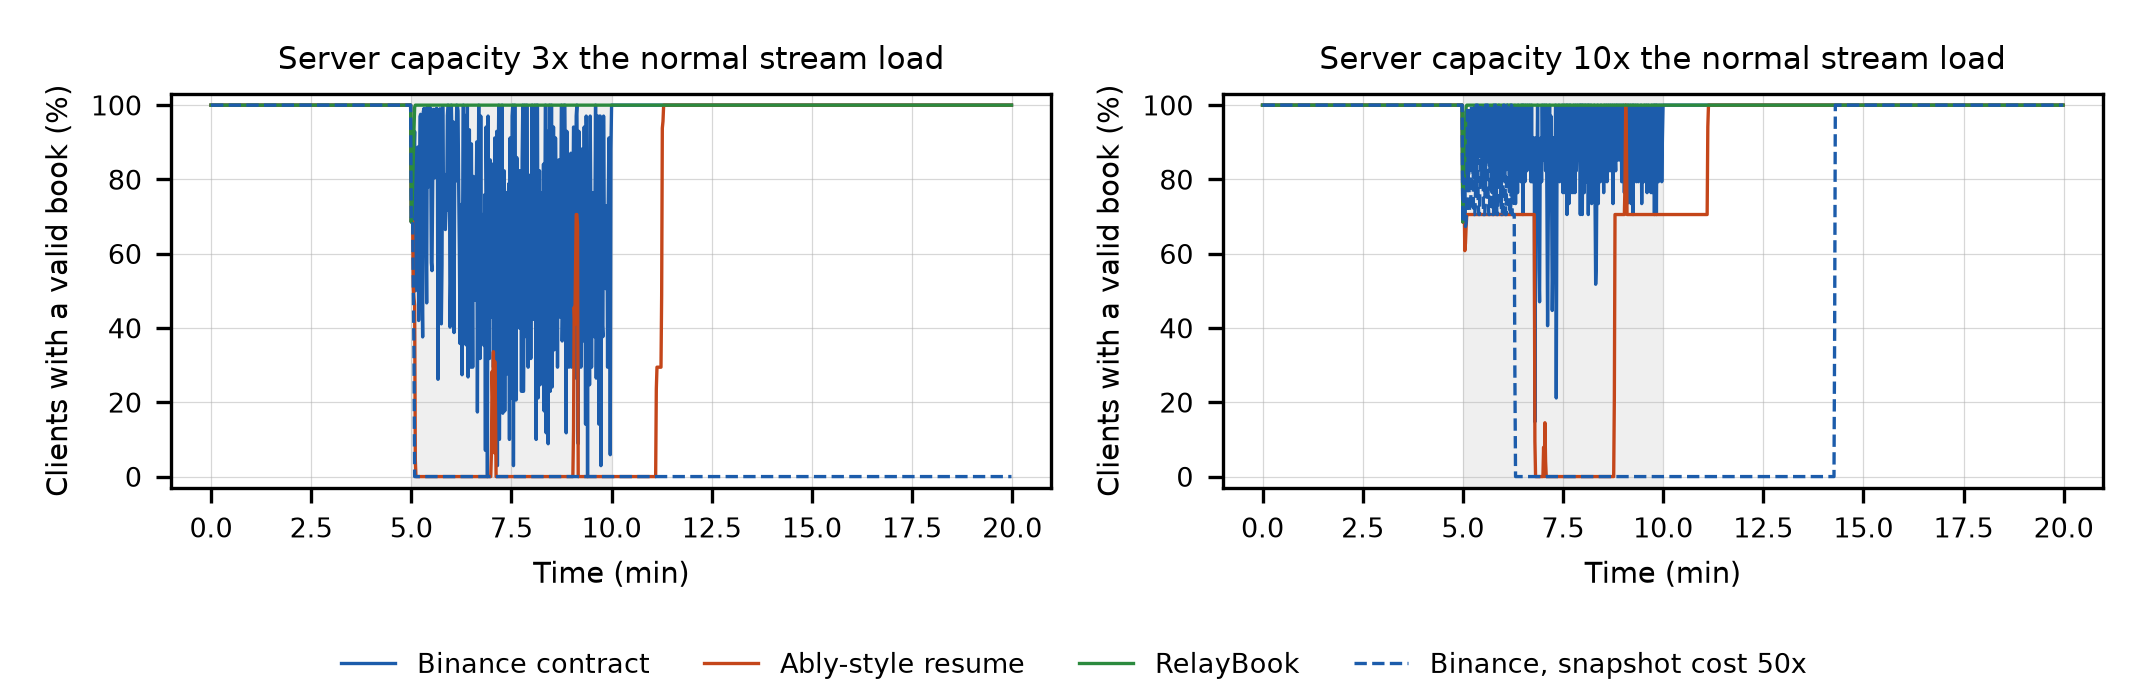
\includegraphics[width=\textwidth]{e2_valid.png}
\caption{Share of clients with a valid book, averaged per second. The shaded interval is the spike at 10x.}
\label{fig:valid}
\end{figure*}

\begin{figure}[t]
\centering
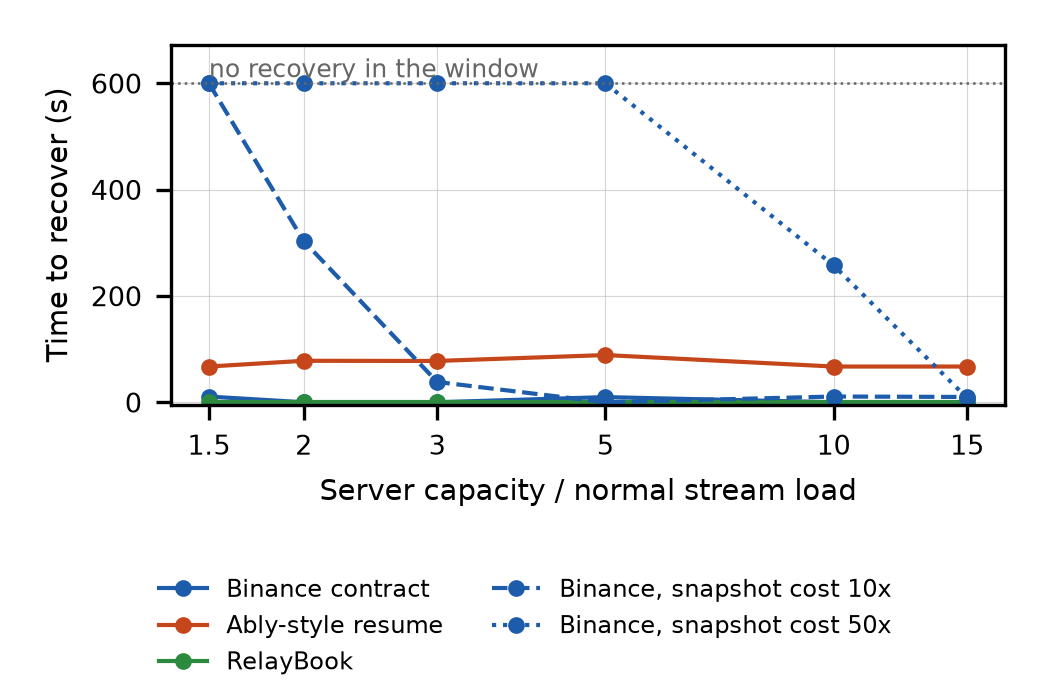
\includegraphics[width=\columnwidth]{e2_ttr.png}
\caption{Time to recover after the spike across server capacities and snapshot costs.}
\label{fig:ttr}
\end{figure}

\section{Discussion}

The first part of the hypothesis held only under some conditions. The public Binance contract remained degraded after the spike when generating a snapshot cost at least ten times its bytes and the origin had little spare capacity, and in those cases abandoned requests that were still processed sustained the overload. When a snapshot cost the same as sending its bytes, the contract recovered within seconds. Since the real cost of a snapshot at Binance is unknown, the result locates the conditions under which the public contract is vulnerable rather than confirming a failure in production.

The second part of the hypothesis held for the time to recover and was close for the staleness, which exceeded the 1\,s target by 0.1 to 0.3\,s. It did not hold for the share of full resynchronizations, which reached 100\% during the spike. The measurements explain the difference. The saving of state-based resume over a snapshot exists for short disconnections at normal rate, while during a spike the changed levels saturate the book within a second. The improvement of RelayBook therefore came from where the recovery happens and from conflation, which kept the origin load independent of disconnections and prevented slow clients from losing their connection, rather than from smaller recoveries. Against a log-based resume, state-based resume reduced the payload by a factor between 3 and 84 depending on the duration of the disconnection.

The results are subject to several threats. The simulator models network capacity but not processing cost, which motivated the sweep of the snapshot cost. The evaluation used a single instrument, a single recording of 70 minutes and a replay at 10x as a surrogate for a volatility spike. The client behavior, such as the 5\,s staleness threshold and the 10\,s retry, follows common practice but varies across real clients. The Ably-style baseline reproduces the documented resume window and not the full Ably service, and the internal mitigations of Binance remain unknown.

\section{Conclusion}

RelayBook moves the recovery of market data clients from the origin to regional relays and resumes clients from the state of the book. On real Binance traffic, the relay recovered every client with a correct book, and state-based resume reduced the recovery payload for short disconnections and by a large factor against a log-based resume. In a simulated reconnection storm, RelayBook returned to a healthy state immediately and kept the origin load independent of disconnections, while the public Binance contract failed to recover only when snapshots were expensive for the origin. The hypothesis was refuted for the share of full resynchronizations during a spike, which shows that the benefit of the architecture lies in where recovery happens rather than in the size of each recovery. Future work includes measuring the cost of snapshots, evaluating several instruments and deploying relays over a real network.

\section*{Use of AI Tools}

Claude (Anthropic) was used to support the literature search and the drafting of this document. The authors selected the problem, verified the sources and made the final decisions.

\bibliographystyle{IEEEtran}
\bibliography{referencias}

\end{document}
